\documentclass[11pt,twoside=true]{scrartcl}
\usepackage[utf8]{inputenc}
\usepackage[english]{babel}
\usepackage{amsmath,amsthm,verbatim,amssymb,amsfonts,amscd, graphicx}
\usepackage{graphicx}
\usepackage{siunitx}
\usepackage{mhchem}
% \usepackage[T1]{fontenc}
% \usepackage{charter}
\usepackage[bitstream-charter]{mathdesign}
\usepackage[hyperref=true,
            url=false,
            isbn=false,
            backref=true,
            % style=science,
            citereset=section,
            maxcitenames=3,
            maxbibnames=100,
            block=none,
            backend=biber]{biblatex}

\addbibresource{sources.bib}

%% MATH COMMANDS
\newcommand{\dd}[2]{\frac{d{#1}}{d{#2}}}

\usepackage[%
  bookmarks, % Create bookmarks
  bookmarksopen=true, % Unfold bookmatk tree in PDF viewer when document is opened
  bookmarksopenlevel=1, % Level of unfolding
  bookmarksnumbered=true, % Number bookmarks
  hidelinks, % do not highlight hyperlinks -- looks ugly
  pdfpagelabels=true, % See manual...
  plainpages=false, % See manual...
  hyperfootnotes=true, % Hyperlinks for footnotes
  hyperindex=true, % Indexeinträage verweisen auf Text
]{hyperref}


\setkomafont{section}{ \LARGE\bf }
\setkomafont{title}{ \Large\bf }
\setkomafont{section}{ \Large\bf }
\setkomafont{subsection}{ \normalfont\bf }



\titlehead{
    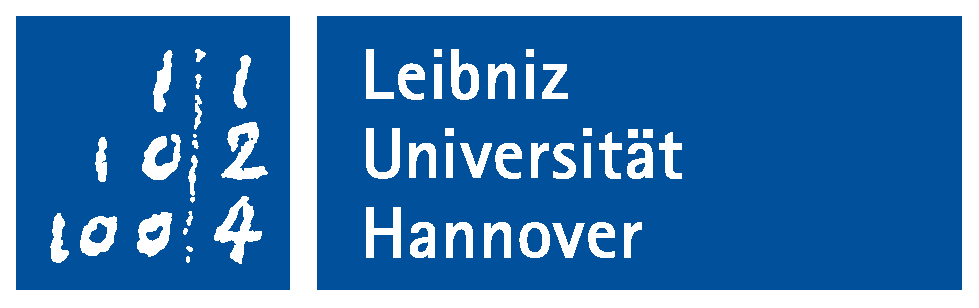
\includegraphics[width=5cm]{./figures/luh_logo.eps}
  
}
\title{Praktikumsbericht}
\subtitle{Erzeugung ultrakurzer Laserpulse (IQ 7)}
\author{Jonathan Rossberg,
      Eduard Sauter}
\date{\today}
\dedication{Praktikum im Rahmen der Vorlesung Koheränte Optik im
Sommersemester 2016}


\begin{document}

\maketitle

\section{Theory}
\textsl{Bestimmen sie den theoretischen Verlauf der $g_0-P$ Kennlinie} 
%
Die Ratengleichungen lauten.
\begin{align*}
  T_R \dd{g}{t} & 
    = \underbrace{\frac{g_0}{T_L}}_{\text{Pumpen}}   
    - \underbrace{\frac{g P}{ P_{\text{sat}}}}_{\text{Stimulierte Emission}}  
    - \underbrace{\frac{g}{T_L}}_{\text{Dunkle Abregung}} \\
  T_R \dd{P}{t} & 
    = \underbrace{2 g P}_{\text{Stimulierte Emission}}  
    + \underbrace{2 g P_\text{vac}}_{\text{Spontane Emission}}  
    - \underbrace{\frac{P}{T_p}}_{\text{Lineare Verluste}}
\end{align*}
%

\section{The Potential Well Model}
\begin{figure}[h!]
  \centering
  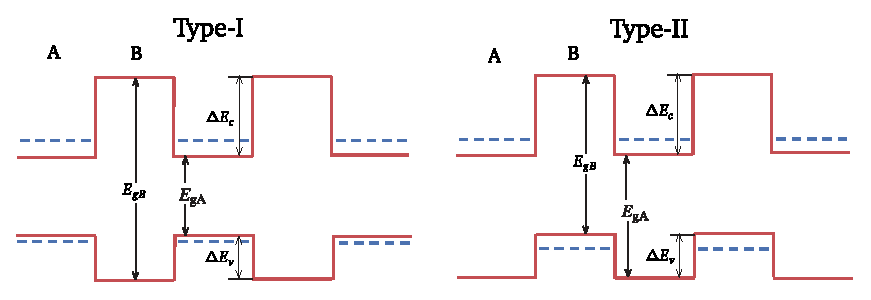
\includegraphics[width=1\textwidth]{./figures/quantum_well_types}
  \caption{Comparison between the different Band Edge alignments in Quantum 
  Wells. Taken from \cite{yucardona}}
  \label{fig:quantum_well_types}
\end{figure}



\section{Type-II Multiple Quantum Wells}
\begin{figure}[h!]
  \centering
  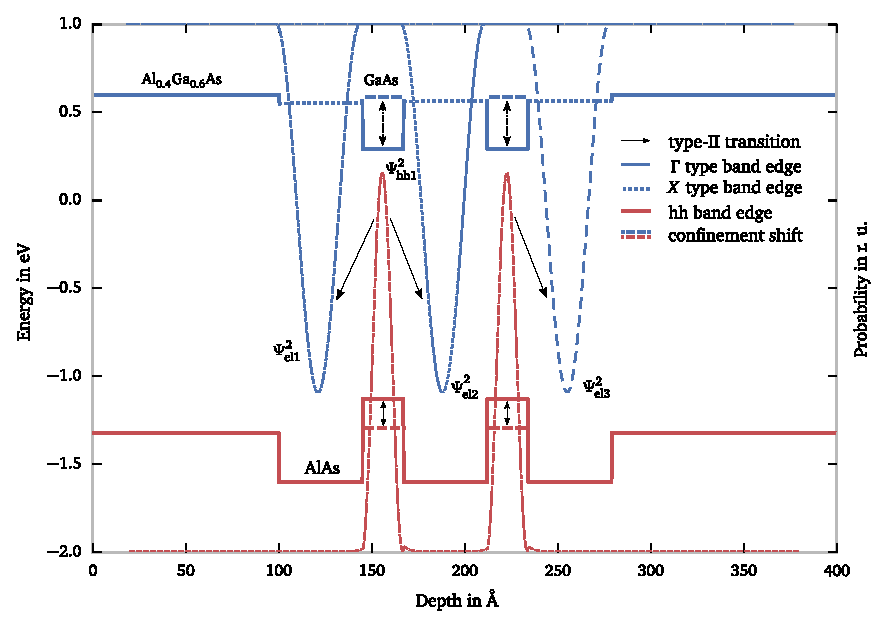
\includegraphics[width=\textwidth]{./figures/samplegaas_spatial_bandstructure.eps}
  \caption{
    Lowest Energy Wave functions of Electrons and Holes with $k$-vectors close to the band edges.
    This figure illustrates the expected spatial separation of the electron
    and hole states. Calculated with \cite{snider19901d}
  } 
  \label{fig:} 
\end{figure}

Ziel dieses Versuchs ist die Messung der Spinrelaxationszeit angeregter
Elektronen in einer n-dotierten \ce{GaAs} Probe bei niedrigen Temperaturen. 
Laut \cite{dzhioev2002low} ist die Spinrelaxationszeit maximal bei einer
Dotierung von etwa \SI{1e16}{\per\cubic\centi\metre}. Die dotierung der
untersuchten Probe liegt auch in diesem Bereich.

Die Beständigkeit des Spins ist interessant für Spintronische Anwendungen. Dort
wird der Spin verwendet, um Informationen zu manipulieren, zu speichern und
wieder abzurufen. Es ist von Vorteil, wenn diese Informationen nicht zu schnell
verloren gehen.

Die Spinrelaxationszeit wird hier mithilfe einer \emph{Hanle-Messung} bestimmt.
Andere mögliche Bestimmungsverfahren sind zum Beispiel Spinrauschspektroskopie oder
Zeitaufgelöste Messung.


\section{Theorie}

Im Grenzfall geringer Bestrahlungsdichten werden nur wenige Elektronen durch
das zirkular polarisierte Licht angeregt, und folglich gibt es wenig 
Rückkombination der entstehenden Löcher mit den optisch angeregten Elektronen.
Vielmehr rekombinieren die Elektronen mit den reichlich vorhandenen 
unpolarisierten Gleichgewichtselektronen \footfullcite{dzhioev2002low}. 

Zusätzlich stehen Übergangswahrscheinlichkeiten vom $p$-Artigen Valenzband bei
Anregung mit $\sigma_+$ oder $\sigma_-$ für den Übergang in die Zustände $s =
\pm\frac{1}{2}$ des Leitungsbandes stehen in einem Ungleichgewicht. 

Durch diese beiden Faktoren kann sich letztendlich ein Gleichgewicht einstellen,
in dem es eine gewisse Ansammlung von Gesamtelektronenspin im Leitungsband gibt.

Unter Einfluss des Magnetfeldes erwarten wir aufgrund der \emph{Larmor-Präzession}
eine sich zeitlich veränderliche Projektion des Spins der Elektronen senkrecht
zum angelegten Magnetfeld $B$ mit der \emph{Larmor-Frequenz}
\begin{align*}
  \Omega(B) = \frac{g \mu_B B }{\hbar}
\end{align*}
%
Wir erwarten dann, dass die Gesamtpolarisation
der Photolumineszenz dem Verlauf einer \emph{Hanle-Kurve} entspricht
\cite{fpspindynamik}.
%
\begin{align*}
  \bar{S}_Z(B) = \frac{\bar{S}_Z(0)}{1 + \left( \frac{T_S g \mu_B B}{\hbar} \right)^2}  
\end{align*}
%
Wobei wir für das Interpolieren der Messwerte folgende Form verwenden
%
\begin{align*}
  \frac{\bar{S}_Z(0)}{1 + \frac{(B - \Delta B)^2}{\xi^2}} + \Upsilon 
\end{align*}
%
Die Verschiebung der Magnetfeldwerte $\Delta B$ könnte zum Beispiel 
durch das nicht kompensierte Erdmagnetfeld erzeugt werden.

Die \emph{Spinlebenszeit} ist proportional zur Breite der Kurve.
%
\begin{align} 
  T_S = \left( \frac{1}{\tau_s} + \frac{1}{T} \right)\approx \tau_s
  \label{eq:spinrel}
 \end{align} %
Die letztere Näherung verwenden wir nach \cite{dzhioev2002low} unter
der Annahme niedriger Bestrahlungsdichten.
%
Es ergibt sich dann nach \cite{fpspindynamik}
%
\begin{align*}
  \tau_S = \frac{\hbar}{g \mu_B \xi}
\end{align*}
%
Außerdem sind die Naturkonstanten \cite{mohr2012codata}:
%
\begin{align*}
  \mu_B &= \SI{9.27400968(20)e-24}{\joule\per\tesla} \\
  \hbar &= \SI{1.054 571 800(13)e-34}{\joule\second} \\
\end{align*}
%
und der \emph{Landé-Faktor} in \ce{GaAs} bei niedrigen Temperaturen $T \to 0$ 
wird aus \cite{zawadzki2008temperature} entnommen.
%
\begin{align*}
  g = -0.452 
\end{align*}
%
\section{Messaufbau}

Die Probe wird innerhalb eines Krystostaten auf niedrige Temperaturen
abgekühlt. Zum abkühlen wird natürliches, flüssiges Helium verwendet. Eine
Turbomolekularpumpe erzeugt, unterstützt von einer Scrollpumpe, einen Druck
im Größenbereich von \SI{e-8}{\milli\bar}.

Der Laser arbeitet bei einer Wellenlänge unterhalb des direkten Band\-übergangs
von \SI{815}{\nano\metre} ohne energetisch größere Übergänge der $s$-Artigen
Valenzbandniveaus zu ermöglichen.  Um Wellenlängen über der Bandlücke zu
unterdrücken schalten wir einen Niedrigpass Filter vor den Laser. Sie könnten
bei der Messung störend sein, falls sie von der Probe reflektiert werden und
durch den Hochpass Filter vor der Diode geraten. Der Hochpass Filter soll
Reflexe niedriger Wellenlänge, welche vom Laser ausgehen können, unterdrücken.
Zwei Justierspiegel ermöglichen die Ausrichtung des Strahlengangs auf die Höhe
der Probe. 

Um einen größeren Bereich der Probe mit geringerer Strahlungsdichte
auszuleuchten wird der Laserstrahl mit einer Linse aufgeweitet.

Die Achse des PEM wird im \SI{45}{\degree} Winkel zum Linearpolarisator
ausgerichtet und moduliert so unter Wechselspannung die Polarisation des
Laserstrahls Sinusförmig zwischen $\sigma_-$ und $\sigma_+$.

Die Photolumineszenz wird durch eine $\lambda/4$ Platte gesendet, und so kann
aus der Amplitude ihres durch den PEM modulierten Intensitätsverlaufes ihre
Gesamtpolarisation bestimmt werden.

Der photoelastische Modulator, ein doppelbrechender Kristall, der mit einer
Frequenz von \SI{50}{\kilo\hertz} zusammengedrückt und ausgedehnt wird und bei
maximaler Ausdehnung als $\lambda/4$-Plättchen wirkt, erzeugt die Oszillationen
von links- und rechtszirkular polarisiertem Laserlicht. Damit oszilliert auch
das Photoluminiszenzsignal zwischen links- und rechtszirkular polarisiertem
Licht.  Dazu wird nur eine Komponente $\sigma_+$ oder $\sigma_-$ bei der
Messung berücksichtigt. Sie wird durch den Linearpolarisator 2 herausgefiltert.

Die Amplitude wird direkt mit dem Lock-In Amplifier gemessen, der seine Lock-In
Frequenz durch den PEM erhält.  Er verstärkt schließlich das Signal und
unterdrückt gleichzeitig Rauschanteile durch einen DC-Filter. Das Signal des
Lock-Ins wurde am Computer gleich ausgewertet.

Die Probe selbst befindet sich in einem 4He-Metall-Dewargefäß, an dessen äußere
Kammer zwei Vakuumpumpen angeschlossen sind. In der inneren Kammer tropft
flüssiges Helium auf einen Kupferfinger, an dem die Probe angebracht ist. Sie
soll diese auf etwa \SI{6.5}{\kelvin} herunterkühlen.  Ein Computer regelt die
Stromversorgung der Helmholtz-Spule, welche vorher durch ein Gauss-Meter
kalibriert wurde. Er nimmt auch die Amplitudenwerte des Lock-In auf und erzeugt
auf diese Weise die Messreihen des nächsten Abschnittes.  





\section{Messergebnisse}
Unsere Messungen der Spinpolarisation in Abhängigkeit vom Magnetfeld liefern
uns die Hanle-Kurve, welche in der untenstehenden Abbildung dargestellt ist. In
einer ersten Messung, dargestellt in der unteren der beiden Kurven, haben wir
bei einer Laserintensität von \SI{22.5}{\milli\watt} 50 Messwerte aufgenommen
und jeweils die Stromstärke um \SI{100}{\milli\ampere} erhöht. In einer zweiten
Messung wurden je 50 Messwerte in kleineren Abständen von
\SI{80}{\milli\ampere} in beide Polungsrichtungen gemessen (oberes Diagramm).
Die Halbwertsbreiten der Hanle-Kurven der beiden Messungen liefern uns
schließlich über Gleichung \ref{eq:spinrel} die Spinrelaxionszeit.
$
\tau_{s_1}=\SI{20.199 \pm 1.344}{\nano\second}
$
für die erste Messung und
$
\tau_{s_2}=\SI{25.535 \pm 0.429}{\nano\second}
$
für die zweite Messung.

Die beiden Messungen hätten bei einer Temperatur von \SI{6.5}{\kelvin}
stattfinden sollen. Da das Kryostat eine fehlerhafte Dichtung hatte, ist diese
Temperatur allerdings nicht erreicht worden. Geplant waren ursprünglich auch
noch zwei weitere Messungen mit verschiedenen Laserintensitäten. Da bei einer
Überprüfung, ob ein Leck vorliegt, schießlich das Vakuum komplett
zusammengebrochen ist, wurden diese beiden Messungen nicht mehr durchgeführt.





\section{Diskussion der Ergebnisse}
Wie man sieht lassen sich unsere Messdaten der Theorie entsprechend sehr gut
durch eine Lorentz-Kurve approximieren. Vor allem die zweite Messung, in der
wir die Stromstärke in kleineren Abständen verändert haben, zeigt geringe
Abweichungen von deren Verlauf. Allerdings fehlen hier bei
der Messung in negativer Stromrichtung die ersten zwei Messwerte, da die
Sättigungsgrenze des Lock-Ins erreicht war. 

Anhand der Halbwertsbreite der Hanle-Kurve haben wir also die Spinlebenszeit
von etwa \SI{23}{\nano\second} bestimmen können. Aufgrund bisheriger
Erfahrungen mit dem Versuchsaufbau wären allerdings Lebenszeiten
im Bereich von bis zu \SI{100}{\nano\second} erwartet worden. Da allerdings
aufgrund der fehlerhaften Dichtung die Temperatur der Probe \SI{6.5}{\kelvin} 
vermutlich deutlich überschritten hat, führte Streuung der Elektronen an
Phononen und Fehlstellen aufgrund der höheren Temperatur zu einer Verringerung
von $\tau_s$ \cite{wu2010spin}.

Auffällig ist überdies die große Verschiebung
$\Delta$B der Hanle-Kurve um den Nullpunkt in beiden Messungen. 
%
Das Erdmagnetfeld wurde nicht kompensiert. Im schlimmsten Fall steht der
magnetische Feldvektor in der Ebene senkrecht zum von der Probe reflektierten
Strahl. Sein Betrag in Deutschland ist etwa \SI{50}{\micro\tesla}. Selbst im
schlimmsten Fall wäre dieser Effekt also zu klein.
%
Wir vermuten daher, dass sich wegen vorangegangenen Anlegens eines Magnetfelds
eine Remanenz in der Probe gebildet haben könnte. Vor allem die erste Messung,
in der $\Delta$B besonders hoch ist, unterstützt diese These. Vor Aufnahme
dieser Messdaten hatten wir mehrmals ein Magnetfeld in gleicher Richtung
angelegt.

\printbibliography


\end{document}
